% F089｜even 原创简明教学示意图
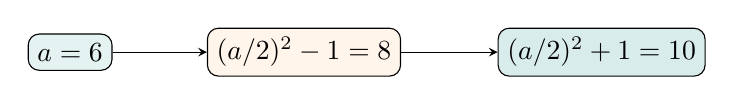
\begin{tikzpicture}[>=stealth,scale=.9]
\node[draw,fill=teal!10,rounded corners] (a) at (0,0){$a=6$};
\node[draw,fill=orange!8,rounded corners] (b) at (3.3,0){$(a/2)^2-1=8$};
\node[draw,fill=teal!15,rounded corners] (c) at (7.5,0){$(a/2)^2+1=10$};
\draw[->] (a)--(b);\draw[->] (b)--(c);
\end{tikzpicture}
